\section{Approach} \label{Sec:approach}
\begin{figure}[!t]
  \centering
  \includegraphics[width=1\hsize]{fig/approachDiagram}
  \vspace{-0.3in} 
  \mycaption{Overview of our assertion generation approach.}
  \label{Fig:approachDiagram}
  \vspace{-0.2in} 
\end{figure}
\IncMargin{0em}
\begin{algorithm}[t]
{\scriptsize
\SetKwInOut{Input}{input}\SetKwInOut{Output}{output}
\Input{Test suite $T$; The set of test cases $tc_i \in T$}
\Output{The ordered set of oracles $oracle$}
\BlankLine

\Begin {
\nl \For{$tc_i \in T$}{
\nl	 $trace\left textsc{Exec}(tc_i)$\\
\nl	 $domAccss\left \textsc{GetDomAcc}(trace)$   	


}

\caption{Oracle Generation} \label{Alg:algorithm}
}
\end{algorithm}
%\DecMargin{lem}
An overview of our unit-level assertion generation technique is depicted in \figref{approachDiagram}.
At a high level, our approach generates unit-level assertions by utilizing human written DOM-based tests and assertions. Our code level assertions fall in the following three categories: (1) explicit assertions, which are directly inferred from analyzing the manually written DOM-based assertions, (2) implicit assertions, which are indirectly affected by the human written DOM-based assertions, and (3) candidate assertions, which are not considered in the written DOM-based assertions, yet are potentially useful to be checked by the function level test suite. We describe our approach below. The numbers below in parentheses correspond to those in the boxes of \figref{approachDiagram}.

In the first part of our approach we (1) execute the instrumented application by running the existing DOM-based test suite. In this step we gather a detailed execution trace of the application. We then extract (2) DOM-based assertions, and (3) candidate DOM element properties, which are useful DOM properties that can potentially be utilized for the purpose of assertion generation. We (4) identify the initial point of connection between the application's source code and checked DOM element. 
%We collect lines of code responsible for updating the corresponding DOM element. 
%We determine DOM mutating statements, 
We (5) calculate the backward slice of the DOM mutating statements to find the entire code blocks that update the checked DOM element. We then (6) extract accessible entities from the obtained statements. Accessible entities form our explicit assertions (7). We further (8) perform a forward slice on the extracted entities to identify statements, that are implicitly affected by such entities. The accessible entities associated with the collected statements form our implicit assertions (9). In addition to explicit and implicit assertions, we also generate candidate assertions (10). Candidate assertions are involved with updating potentially useful DOM element properties, which are not checked in the existing DOM-based assertions. To obtain candidate assertions, we perform step (4), (5), and (6) on the inferred candidate DOM element properties (3).

Our overall unit-level assertion generation is presented in \algref{algorithm}. In the following sections we describe our technique for extracting DOM related information from the execution (\secref{extractDomRelatedInfo}), relating
DOM mutations to the \javascript code (\secref{domToCode}), and generating unit test assertions (\secref{unitLevelAssertion}).   
\subsection{Extracting DOM-Related Characteristics} \label{Sec:extractDomRelatedInfo}
The DOM connects a test case to the web application's code. Therefore, we first need to analyze the DOM-based test suite and extract the following pieces of information: (1) DOM-related operations of the existing test suite that may have tight connection with the \javascript code, and (2) frequently accessed DOM properties, which are potentially influential in improving the fault finding capability of the test suite, but left unchecked in the manually-written test suite.
\headbf{DOM-Related Operations}
Any written test case needs to check the correctness of the application's behaviour. In a DOM-based test case the expected behaviour is checked through DOM-based assertions.
DOM-based assertion is defined as $<domProps,expVal>$, where $domProps$ consists of one or more DOM element features (e.g. attribute, and/or textual value), and $expVal$ is the correct value expected by the assertion. Through the rest of the paper, we call DOM element feature as DOM property. 
DOM-based assertions play a significant role in our approach as they can guide us towards important portions of the underlying \javascript code that need to be checked in unit-level assertions.
\begin{figure}[!t]
  \centering
  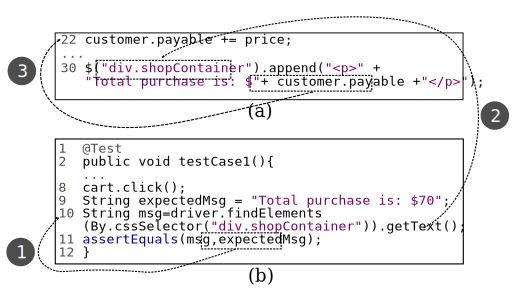
\includegraphics[width=1\hsize]{fig/intraDOMDep}
   \vspace{-0.2in} 
  \mycaption{Finding (1) intra DOM assertion dependency within the test case (b), (2) inter DOM assertion dependency between (b) DOM-based assertion and (a) the \javascript code, and (3) the initial point of contact between (b) DOM-based assertion and (a) the \javascript code.}
  \label{Fig:assertionToCode}
%  \vspace{-0.1in} 
\end{figure}
For each DOM-based assertion we find \emph{intra DOM assertion dependency} within the test case.
\begin{mydef}[Intra DOM Assertion Dependency]
An intra DOM assertion dependency is defined as $<assert, domElems, domProps>$, where $assert$ is the intended DOM-based assertion, $domElems$ is the accessed DOM elements in the test case pertaining to the assertion, and $domProps$ is the accessed DOM properties within the assertion.
\end{mydef}
\textsc{GetDomAcc} in line 10 of \algref{algorithm} retrieves DOM dependencies of the assertion in the test case.
%, we instrument the test case by wrapping around method calls that accesses DOM elements.
Going back to our example in \figref{assertionToCode}(b), tracking the assertion in line 11 shows that it has a DOM dependency to a \code{div} element with class \code{shopContainer}, which is accessed in line 10. The intra DOM assertion dependency of the example further shows that the \code{text} value of the DOM element is compared with the \code{expectedMsg} in line 11.    

We further need to correlate the inferred intra DOM assertion dependency with the application's code.
We call the correlation between the DOM-based assertion and the application's code as \emph{inter DOM assertion dependency}.
\begin{mydef}[Inter DOM Assertion Dependency]
An inter DOM assertion dependency is defined as\\
$<assert, initPoint>$, where $assert$ is the intended DOM-based assertion, and $initPoint$ is the initial line of code in the application that is responsible for mutating the property of a DOM element extracted from the intra DOM assertion dependency.
\end{mydef}
In order to find the initial point of contact between the application's code and a mutated DOM property in the DOM-based test case, we track evolution of the accessed DOM elements (\textsc{GetDomMuts} in line 13 of the algorithm) as well as invoked event handlers as the test case runs. 
We consider additions and removals of child nodes, changes to attributes, and updates to child text nodes as DOM mutations. For instance, running the sample test case in \figref{example}(b) results in mutating (1) the textual value of \code{div} element with class \code{shopContainer}, and (2) the \code{class} attribute of DOM element with ID \code{couponButt}.

In \secref{domToCode}, we explain inferring the initial point of contact between the source code and a mutated DOM element in a DOM-based test suite in details.  
%We call the correlation between the DOM-based assertion and the \javascript code of the application as \emph{inter DOM assertion correlation}. This correlation is defined as $<AccDOMDep, InitCode>$, where $InitCode$ is the initial point of contact in the application's code segment, that is responsible for mutating the previously extracted DOM elements from the test suite ($AccDOMDep$).  
%We make use of \code{document.onload} event to log the initial DOM state. 
%An observer module is then used to monitor mutations on the DOM during the test case execution. 
%In addition to DOM changes, we also keep track of \javascript events as well as invoked event handlers. This information is later used to find the initial point of contact between a DOM mutation and the executed code segments.
%For instance, running the sample test case in \figref{example}(b) results in mutating (1) the textual value of \code{div} element with class \code{shopContainer}, and (2) the \code{class} attribute of DOM element with ID \code{couponButt}.
\headbf{Frequently Accessed DOM Properties}
In addition to DOM-based assertions, we further consider DOM element properties, that are frequently accessed within the application as the test case runs (lines 1 to 7 of \algref{algorithm}). 
\textsc{Acc} in line 6 of the algorithm computes the access frequency of a DOM property, $freqAccdDOM$ in line 7 contains the inferred candidate DOM properties, and \textsc{GetDomMuts} in line 19 records DOM mutations occur
on candidate DOM properties.
The intuition is that frequent use of a given DOM property can point to the extent of application's behaviour dependency on the DOM property. Thus, if changes happen to that property through the \javascript code, it is important to assert the correctness of such mutations. We define the access frequency of a DOM element property as the number of times that the element's property has been read during the execution of a test case. DOM properties include attributes as well as textual value of the elements.
In order to record DOM property accesses within the application, we rewrite native function calls used by programmers to access DOM element such as \code{getElementById}, \code{getElementsByClassName}, and/or \code{getElementsByTagName}. The returned object from these functions is later used to access attributes or textual values of the element. Thus, we apply a forward slice on the returned object to find instances of element's property access in the code.
For example in function \code{addToCart} of \figref{example}(a), DOM element with ID \code{couponButt} is assigned to \code{coupElem} variable. The assigned variable is later used to access the \code{class} attribute as well as the \code{value}
of the DOM element in lines 23, 25, and 26.

Let $Acc(prop_{el})$ be the access frequency computed for property $prop$ of DOM element $el$, then:
 
$Acc(prop_{el})=\frac{Read(prop_{el})}{\sum _{e=1}^{n} Read(domElem_e)}$, where $Read(domElem_{e})$ is the number of times that DOM element $domElem$ is read, given that the total number of DOM elements during the execution of a test case is $n$.
Note that reading a DOM element refers to accessing the element to read the corresponding property. In \figref{example}(a), the \code{class} attribute of DOM element \code{couponButt} is read in lines 23 and 34, and thus the access frequency
computed for the \code{class} attribute of the element is equal to $\frac{2}{3}$.

We choose element's property with access frequencies above a threshold $\alpha$ as potential candidates, which are later used for the purpose of unit-level assertion generation. We automatically compute this threshold for each test case as: 

$\alpha=\frac{1}{ReadProperties(T)}$, where $ReadProperties(T)$ is the total number of properties which have been read during the execution of test suite $T$.

Going back to our running example and the sample DOM-based test case in \figref{example}, \code{class} attribute of the \code{couponButt} is selected as a potential candidate since its access frequency ($\frac{2}{3}$) is greater than the computed threshold, which is equal to $\frac{1}{2}$ in this example.        
%application instrumentaion native event wrapping    

\subsection{Relating DOM changes to the \javascript Code} \label{Sec:domToCode}
To determine the initial point of contact between DOM and the underlying \javascript code, we first cross reference the relevant DOM element with a set of DOM mutations obtained from the execution trace. Our execution trace contains information about the invoked functions, triggered events, as well as DOM mutations caused by the events as the test case runs. This way we can identify relevant events and functions corresponding to a DOM mutation. To figure out where the mutation originated in our execution trace we keep record of DOM accesses within the application. For each DOM access we track \javascript lines of code, that are responsible for updating the corresponding DOM element. After inferring DOM mutant statements within the code, we perform backward slice on the retrieved statements to gather the entire set of \javascript statements responsible for mutating a given DOM element. 
In order to capture dependencies exercised at run-time we use dynamic slicing. We first intercept and statically instrument those statements that may affect a given DOM element. The instrumented code keeps track of all updates and accesses to all relevant data and control dependencies. This trace is later used to extract a dynamic backwards slice.    
Once the test case runs, we collect traces from the instrumented code. This trace is used for extracting dynamically backward sliced statements.

The slicing technique starts by extracting instances of the initial slicing criteria from the trace. For each \textit{read} operations, the trace is traversed backwards to find the nearest related \textit{write} operation. Once found, the \textit{write} operation is added to the slice under construction. This process is repeated for all the data dependencies related to that write operation. A similar approach is taken for including control dependencies in the slice.
To address aliasing when computing the slice of a variable that has been set by a non-primitive value, we need to consider possible aliases that may refer to the same object. Specifically in \javascript \textit{dot notation} and \textit{bracket notation} is frequently used to modify objects at run time. While static analysis techniques often ignore addressing this issue \cite{Feldthaus:icse13}, we incorporate dynamic analysis in our slicing method. If a reference to an object of interest is saved to a second object's property, e.g. through the use of the \textit{dot notation}, the object of interest may also be altered via aliases of the second object. For example, after executing statement \code{a.b.c = objOfInterest;}, updates to \code{objOfInterest} may be possible through \code{a}, \code{a.b}, or \code{a.b.c}. To deal with such scenarios, our slicing technique searches through the collected trace and adds the forward slice for each detected alias to the current slice for our variable of interest (e.g. \code{objOfInterest}). 

By the end of backward slicing step we collect all the relevant statements to a given DOM element, which re later used to derive test assertions.    
\subsection{Generating Unit-Level Assertions} \label{Sec:unitLevelAssertion}
Through analyzing a given DOM-based test case, we generate unit-level assertions in the following three categories: (1) assertions, which are directly related to a given DOM-based assertion, (2) assertions, which are indirectly affected by a given DOM-based assertion, and (3) assertions that have direct impact on important DOM elements which are not checked by the existing DOM-based assertions. In the following we explain each category in details.
\subsubsection{Explicit Assertions} \label{Sec:explicitAssertions}
After collecting all the statements, that are relevant to a given DOM-based assertion, we extract accessible entities from these statements.
Accessible entities include (1) the function's returned value, (2) the used global variables in that function, (3) the object's property where the object is accessible in the outer scope of the function, and/or (4) the accessed DOM element in that function. Dynamic backward slice of a DOM-based assertion helps to (1) track all statements that contribute to the checked result and as such identify those entities that might have influenced the checked property value of the DOM element, and (2) eliminate unrelated entities which are not involved in the computation that leads to the update performed on the checked DOM element.

Since our dynamic slice is extracted from the program run, we can track all concrete values associated with accessible entities.
During the run of a test case, there might be different instances where a given statement is executed. Different execution instances can lead to different behaviour. Since we are employing dynamic slicing, an instance that leads to the required behaviour, which is verified through the DOM-based assertion, is on the backward slice. Given that the manually-written expected value, that is checked against the DOM's property is valid, the concrete values of related entities in the backward slice are potentially correct unless there exists a masked fault which is concealed in the chain of computations and thus does not propagate to the checked state of the DOM element. We conjecture that fault masking rarely happens in \javascript web applications as it is more prevalent in programs with many small expressions whose results are stored in several intermediate values (we further discuss this in the evaluation section). Therefore, concrete value of an entity in the backward slice can potentially be used as the expected value of the entity in unit-level assertions to test the current version of the application.
%We compare the value of the entity immediately after the relevant statement is executed in the backward slice with the entity's value before the function exits. If value of the entity remains the same, we use it towards the expected value in the unit-level assertion.  
%However, if the entity pertaining to a DOM change is reassigned in the code after the DOM gets updated and before the function exits, then the concrete value of the entity can be used for the purpose of regression testing unless the tester provides the proper expected value.
\subsubsection{Implicit Assertions} \label{Sec:implicitAssertions}
We gather all the statements that explicitly affect the computations relevant to a given DOM-based assertion. While assertions inferred from such statements are inherently important, we further need to consider entities that are implicitly influenced by the checked DOM element in the manually-written test suite. For this purpose we apply a dynamic forward slice on the statements collected from a backward slice of a DOM-based assertion.
%\begin{mydef}[Forward Slicing]
%\label{def:forwardSlicing} 
%A forward slice of a program with respect to a statement $st$ at program point $p$ and set of program variables $V$ consists of all statements and predicates in the program that are affected by the value of variables in $V$ at $p$.
%\end{mydef}
A forward slice with respect to a statement $st$,
indicates how subsequently an operand at $st$ is being used. This can help the tester to ensure that $st$ establishes the expected outcome of the computations assumed by later statements. 
%Given the importance of statements involved in code-level computations of a DOM-based assertion, using forward slice is useful to check that there are no unforeseen effects on the application's behavior by a modification to such statements. 

\begin{figure}[!t]
  \centering
  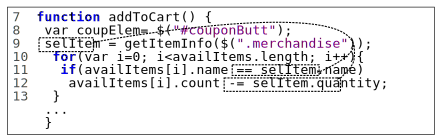
\includegraphics[width=1\hsize]{fig/forwardSlicingExample}
   \vspace{-0.2in} 
  \mycaption{Forward Slicing to obtain implicit assertions.}
  \label{Fig:forwardSlicingExample}
 % \vspace{-0.1in} 
\end{figure}

Dynamic forward slice is performed on the subset of code statements which is previously instrumented as explained in \secref{domToCode}. 
\textsc{GetFWSlice} in line 17 of the algorithm computes forward slice on the variable operands of a statement in the backward slice.
The process of forward slicing is similar to the backward slicing technique discussed earlier (\secref{domToCode}). The slicing criterion of the forward slice module is either a variable, object's property, or an accessed DOM property extracted from the statements in a backward slice segments of the code. The accessible entities (\textsc{Accessibles} in line 24), which have been set within the collected forward slice statements establish the implicit assertions.
$implicitAsstn$ in line 24 of \algref{algorithm} contains the inferred implicit assertions.
\figref{forwardSlicingExample} shows the relevant parts of the code obtained by performing forward slicing on the running example. 
As shown in the figure, the properties of object \code{selItem} are set in line 16, that is recorded during the backward slice process. Given line 16 as the forward slice criteria, we mark \code{availItems.count} (line 19) as an implicit assertion.        
\input{potentialAssertions}
          
%mutation of customer.couponStatus = coupon.Id + '-' + 'used' to customer.couponStatus = coupon.Id + 'used';'